\usetikzlibrary{calc}
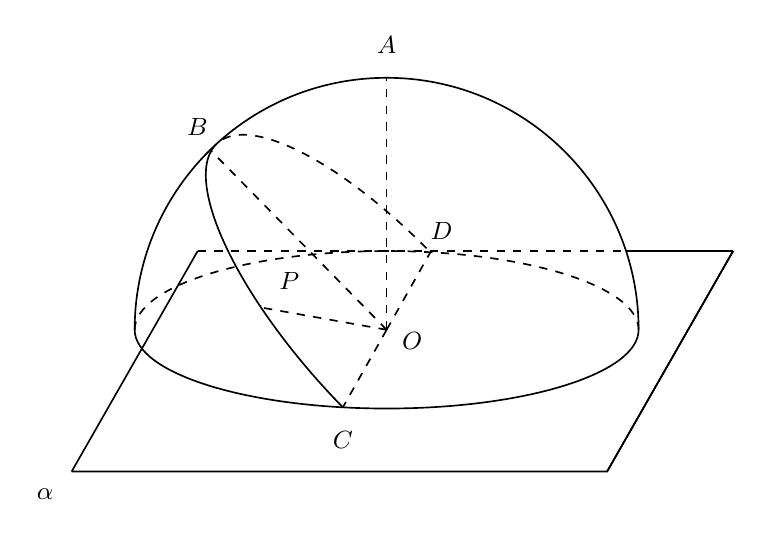
\begin{tikzpicture}[line width=.6pt, font=\small, x=1cm, y=1cm]
\coordinate (P1) at (-3.4,-1.6);
\coordinate (P2) at (3.4,-1.6);
\coordinate (P3) at (5.0,1.2);
\coordinate (P4) at (-1.8,1.2);
\draw (P1)--(P2)--(P3);
\draw (P4)--(P1);
\draw[dashed] (P4)--(3.6397368307,1.2);\draw (3.6397368307,1.2)--(P3);
\draw (P2)--(P3);
\coordinate (O) at (0.6,0.2);
\coordinate (C) at (0.0443258315,-0.7848077530);
\coordinate (Cl) at (-2.6,0.2);
\coordinate (Cr) at (3.8,0.2);
\draw (Cl) arc (180:360:3.2 and 1.0);
\draw[dashed] (Cl) arc (180:0:3.2 and 1.0);
\coordinate (A) at (0.6,3.4);
\draw (Cl) arc (180:0:3.2);
\coordinate (B) at (-1.6283655690,2.4722063300);
\coordinate (D) at (1.1556741685,1.1848077530);
\draw[domain=0:90,samples=80,variable=\t] plot ({.6+-0.555674168534*cos(\t)+-2.228365569024*sin(\t)},{.2+-0.984807753012*cos(\t)+2.272206329989*sin(\t)});
\draw[dashed,domain=90:180,samples=80,variable=\t] plot ({.6+-0.555674168534*cos(\t)+-2.228365569024*sin(\t)},{.2+-0.984807753012*cos(\t)+2.272206329989*sin(\t)});
\draw[dashed] (O)--(A);
\draw[dashed] (O)--(B);

\draw[dashed] (O)--(D);
\coordinate (P) at (-0.9954107307,0.4832346330);
\draw[dashed] (O)--(P);

\node[above=5pt] at (A) {$A$};
\node[left=5pt,above=2pt] at (B) {$B$};
\node[below=5pt] at (C) {$C$};
\node[right=4pt,above=1pt] at (D) {$D$};
\node[below=4pt,right=2pt] at (O) {$O$};
\node[above right=3pt] at (P) {$P$};
\node[below=8pt,left=3pt] at (P1) {$\alpha$};
\draw[dashed] (O)--(C);\end{tikzpicture}
